%%%%%%%%%%%%%%%%%%%%%%%%%%%%%%%%%%%%%%%%%
% Beamer Presentation
% LaTeX Template
% Version 1.0 (10/11/12)
%
% This template has been downloaded from:
% http://www.LaTeXTemplates.com
%
% License:
% CC BY-NC-SA 3.0 (http://creativecommons.org/licenses/by-nc-sa/3.0/)
%
%%%%%%%%%%%%%%%%%%%%%%%%%%%%%%%%%%%%%%%%%

%----------------------------------------------------------------------------------------
%	PACKAGES AND THEMES
%----------------------------------------------------------------------------------------

\documentclass{beamer}

\mode<presentation> {

% The Beamer class comes with a number of default slide themes
% which change the colors and layouts of slides. Below this is a list
% of all the themes, uncomment each in turn to see what they look like.

%\usetheme{default}
%\usetheme{AnnArbor}
%\usetheme{Antibes}
%\usetheme{Bergen}
%\usetheme{Berkeley}
%\usetheme{Berlin}
%\usetheme{Boadilla}
%\usetheme{CambridgeUS}
%\usetheme{Copenhagen}
%\usetheme{Darmstadt}
%\usetheme{Dresden}
%\usetheme{Frankfurt}
%\usetheme{Goettingen}
%\usetheme{Hannover}
%\usetheme{Ilmenau}
%\usetheme{JuanLesPins}
%\usetheme{Luebeck}
\usetheme{Madrid}
%\usetheme{Malmoe}
%\usetheme{Marburg}
%\usetheme{Montpellier}
%\usetheme{PaloAlto}
%\usetheme{Pittsburgh}
%\usetheme{Rochester}
%\usetheme{Singapore}
%\usetheme{Szeged}
%\usetheme{Warsaw}

% As well as themes, the Beamer class has a number of color themes
% for any slide theme. Uncomment each of these in turn to see how it
% changes the colors of your current slide theme.

%\usecolortheme{albatross}
%\usecolortheme{beaver}
%\usecolortheme{beetle}
%\usecolortheme{crane}
%\usecolortheme{dolphin}
%\usecolortheme{dove}
%\usecolortheme{fly}
%\usecolortheme{lily}
%\usecolortheme{orchid}
%\usecolortheme{rose}
%\usecolortheme{seagull}
%\usecolortheme{seahorse}
%\usecolortheme{whale}
%\usecolortheme{wolverine}

%\setbeamertemplate{footline} % To remove the footer line in all slides uncomment this line
%\setbeamertemplate{footline}[page number] % To replace the footer line in all slides with a simple slide count uncomment this line

%\setbeamertemplate{navigation symbols}{} % To remove the navigation symbols from the bottom of all slides uncomment this line
}

\usepackage{graphicx} % Allows including images
\usepackage{booktabs} % Allows the use of \toprule, \midrule and \bottomrule in tables
\usepackage{hyperref,tikz}
\usetikzlibrary{arrows,shapes,matrix,positioning}
\usepackage{chemfig,siunitx}
\setcompoundsep{7em}
\usepackage{algorithm,algorithmic}
%----------------------------------------------------------------------------------------
%	TITLE PAGE
%----------------------------------------------------------------------------------------

\title[RNA circuits]{Self-contained RNA inhibition with trans-cleaving ribozymes} % The short title appears at the bottom of every slide, the full title is only on the title page

\author{Zack Field \& Ryan Tsoi} % Your name
\institute[UC Berkeley] % Your institution as it will appear on the bottom of every slide, may be shorthand to save space
{
University of California \\ % Your institution for the title page
\medskip
\textit{field.zackery@berkeley.edu, ryantsoi@berkeley.edu} % Your email address
}
\date{\today} % Date, can be changed to a custom date

\begin{document}

\begin{frame}
\titlepage % Print the title page as the first slide
\end{frame}

\begin{frame}
\frametitle{Overview} % Table of contents slide, comment this block out to remove it
\tableofcontents 
% Throughout your presentation, if you choose to use \section{} 
% and \subsection{} commands, these will automatically be printed 
% on this slide as an overview of your presentation
\end{frame}

%----------------------------------------------------------------------------------------
%	PRESENTATION SLIDES
%----------------------------------------------------------------------------------------

%------------------------------------------------
\section{Introduction} % Sections can be created in order to organize your presentation into discrete blocks, all sections and subsections are automatically printed in the table of contents as an overview of the talk
%------------------------------------------------

\subsection{Genetic Regulation} % A subsection can be created just before a set of slides with a common theme to further break down your presentation into chunks

\begin{frame}
\frametitle{Promise of Synthetic Biology}

Complexity of eukaryotes $\not\approx$ \# of protein coding genes

\begin{tabular}{l | l | l}
\hline
Oryza sativa (rice)& 470 million & 51,00\\
Gallus gallus (chicken)& 1 billion& 20,000-23,00\\ 
Canis familiaris (dog)& 2.4 billion& 19,00 \\
Mus musculus (mouse)& 2.5 billion& 30,00 \\
Homo sapiens & 2.9 billion& 20,000-25,000\\
\hline
\end{tabular}

\bigskip
The root of biological complexity is believed to be genetic regulation.

However, the creation of novel protein regulatory elements is too difficult.

Re-writers RNA-world may be the key to getting a handle on regulation.           
\end{frame}

%------------------------------------------------

\subsection{Motivation}

\begin{frame}
\frametitle{Motivation}

Toggle switch and repressilator in 2000, to now.
 
\begin{figure}[ht]
  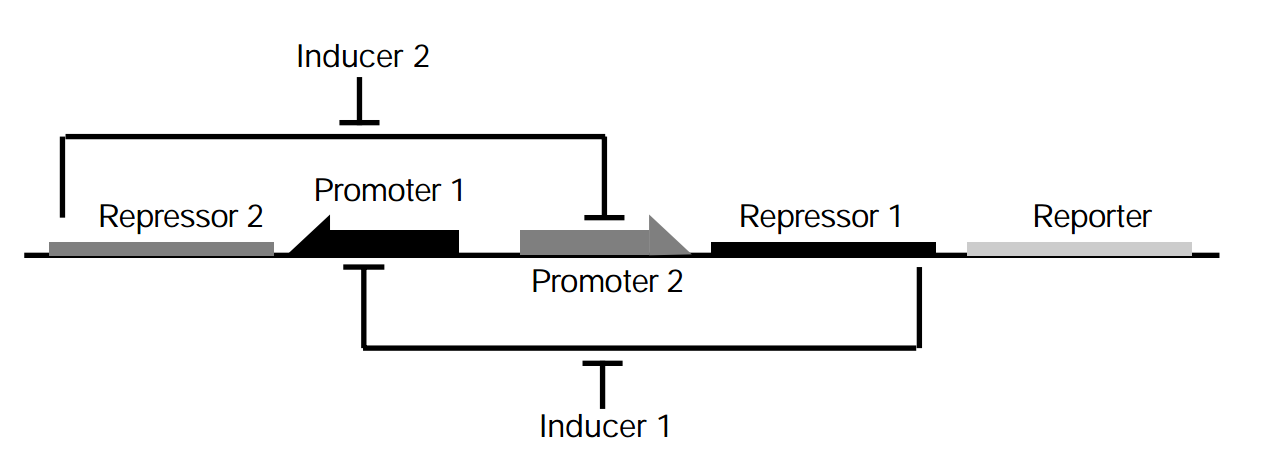
\includegraphics[width=0.5\textwidth]{DNA_toggle.png}
  \hfill
  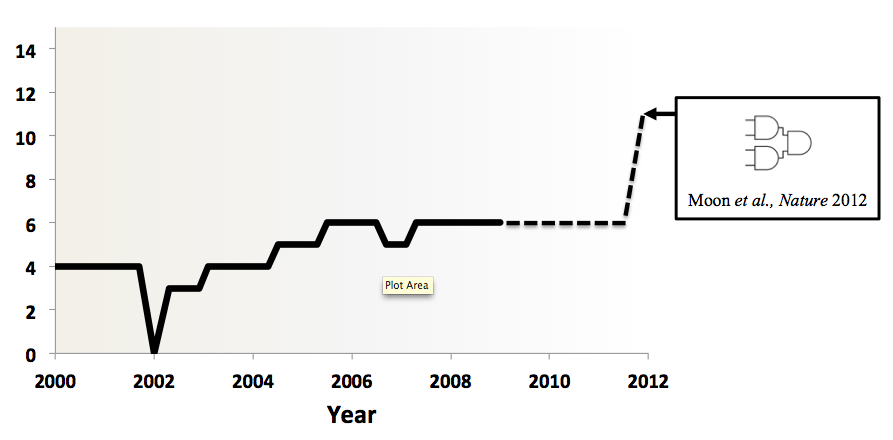
\includegraphics[width=0.5\textwidth]{circuit_complexity.png}
\end{figure}

\begin{figure}[ht]
  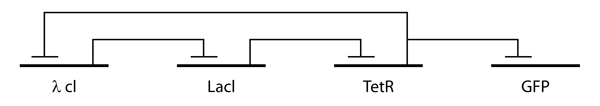
\includegraphics[scale=0.4]{repressilator.png}
\end{figure}
\end{frame}

\begin{frame}
%\frametitle{Motivation}
Exponential decrease in the cost of enabling technologies should result 
in exponential growth of circuit complexity.

\begin{figure}
  \centering
  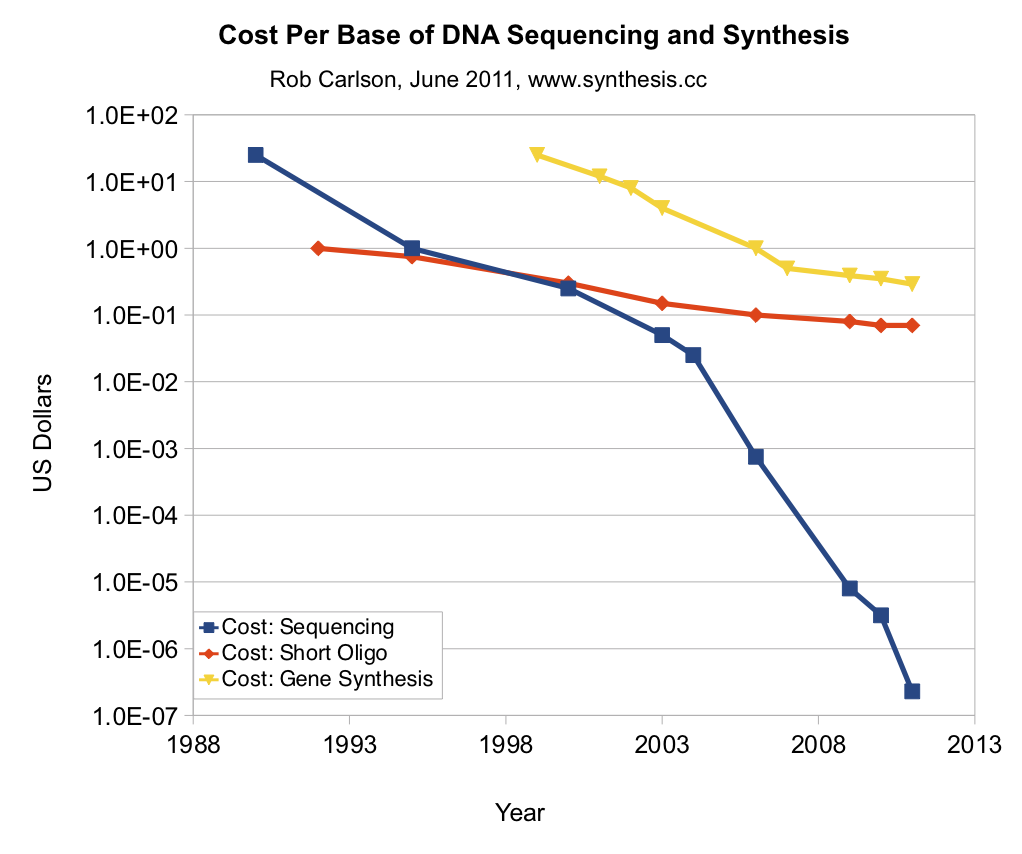
\includegraphics[scale=0.5]{cost_per_base.png}
\end{figure}
\end{frame}

\begin{frame}
\begin{block}{Pitfalls in current promoter-repressor pair design}
  \begin{itemize}
    \item Orthogonal  - Limited number of repressors (until very recently)
    \item Predictable - Gene circuit evolves away
    \item Safe        - shRNA toxicity in gene therapy
    \item Reliable    - 40 hour toggle switch breakdown
    \item Designable  - Protein structure prediction too difficult
    \item Cooperativity - Unpredictable behavior when juxtaposed
  \end{itemize}
\end{block}

\end{frame}

%------------------------------------------------

\subsection{Possible non-coding RNA tools}
\begin{frame}
\frametitle{Signal Transduction with RNA, possible tools}

\begin{figure}
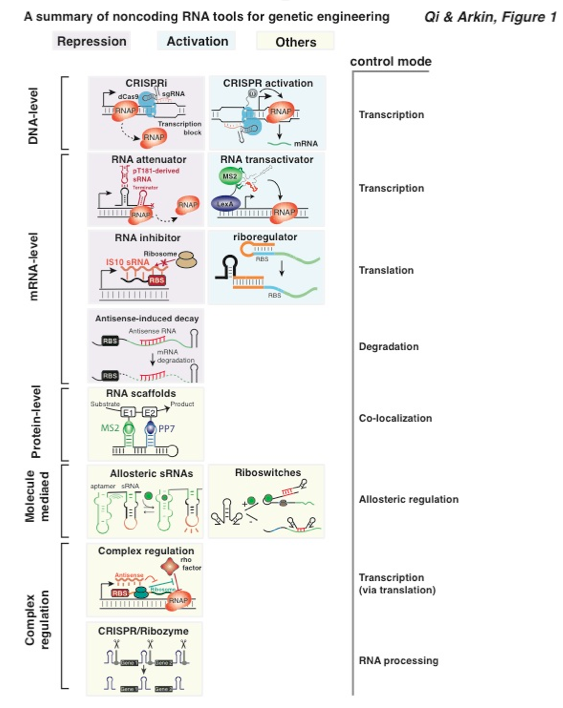
\includegraphics[width=0.5\textwidth]{riboregulation.png}
\hfill
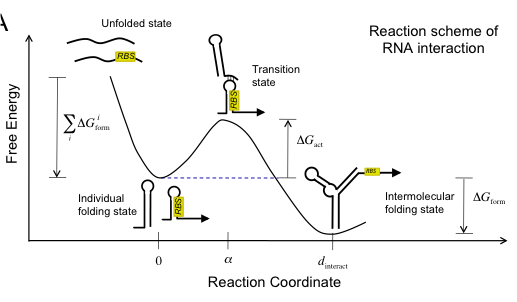
\includegraphics[width=0.45\textwidth]{energy_riboregulation.png}
\end{figure}
\end{frame}

%------------------------------------------------
\section{Riboregulation decision}
\subsection{Choice of ribozyme}


\begin{frame}
\frametitle{Choice of trans-cleaving  hammerhead ribozymes}

Self-contained mechanism of RNA degradation

Composable and functionally complete 

\begin{figure}
  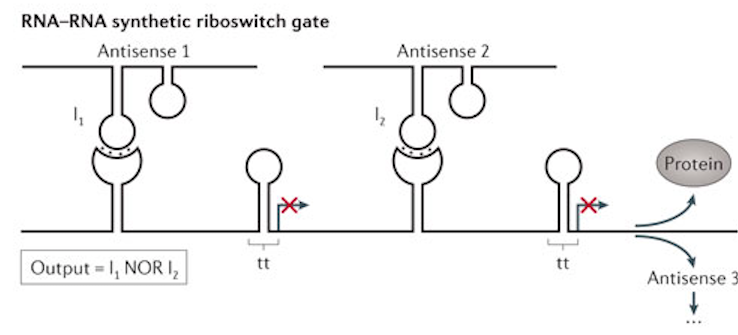
\includegraphics[scale=0.25]{functional.png}
\end{figure}

Base-pairing rather than aptamer coupling for 
ease of rational design

Watson Crick base pairing dominates free energy minimization
\end{frame}

%------------------------------------------------

\subsection{General riboregulation model}
\begin{frame}
\frametitle{General riboregulation model}

Stochastic model - Gillespie algorithm


\begin{algorithm}[H]
\begin{algorithmic}[1]
  \STATE{{\bf Inputs:} }
  \STATE{Set of $M$ reactions and $avg\_Prob[]=c$; $R_i=(c_{i}) i\in{1,\ldots,M}$}
  \STATE{Initial population sizes, $endtime$}
  \STATE{{\bf Output:} Catalog of Molecular events}
  \WHILE{$\tau < endtime$}
  \STATE $a_{0} = 0$
  \FOR{$i=1$ to $M$}
  \STATE $a_{i} = h_ic_i$, where $h_i$ is the amount of reactant
  \STATE $a_0 += a_{i}$
  \ENDFOR
  \STATE $(\tau,\mu) \leftarrow P(\tau,\mu)$
  \STATE updatePopulation($R_{\mu}$)
  \ENDWHILE
\end{algorithmic}
\caption{Gillespie}
\end{algorithm}

\end{frame}

%------------------------------------------------

\subsection{Model and Kinetics of trans-cleaving ribozyme}
\begin{frame}
\frametitle{trans-cleaving ribozyme model and kinetics}

From Samarsky \emph{et al.} 

\scalebox{0.7}{
  \schemestart
  $A_{DNA}$
  \arrow{->[$k_{tc_a}$]}
  $A_{RNA}$
  ,
  $B_{DNA}$
  \arrow{->[$k_{tc_b}$]}
  $B_{RNA}$
  \schemestop
}

\bigskip

\scalebox{0.7}{
  \schemestart
  $A_{RNA} + B_{RNA}$
  \arrow{<=>[$k_1$][$k_{-1}$]}
  $A_{RNA}\cdot B_{RNA}$
  \arrow{->[$k_2$]}
  $A_{RNA}\cdot F_1 \cdot F_2$
  \arrow{->[$k_3$]}
  $A_{RNA}+F_1'$
  \schemestop
}

\bigskip 

All species undergo degradation at some rate $k_{deg}$.

\bigskip

MM kinetics

Fraction of substrate/time: $k_{obs} = k_2 \times [A_{RNA}\cdot B_{RNA}]/[B_{RNA_{0}}]$

$k_3>>k_2>>k_{deg}$ by single orders of magnitude. 

\end{frame}

%------------------------------------------------

%\subsection{Toggle switch model DNA-based}
%\begin{frame}
%\frametitle{Toggle switch model DNA-based}
%
%\end{frame}

%------------------------------------------------

\subsection{Toggle switch model riboregulation}
\begin{frame}
  \frametitle{Toggle switch model riboregulation}

No possible bistable point. First limitation.

\begin{columns}[T]
    \begin{column}{0.5\textwidth}
      \centering
       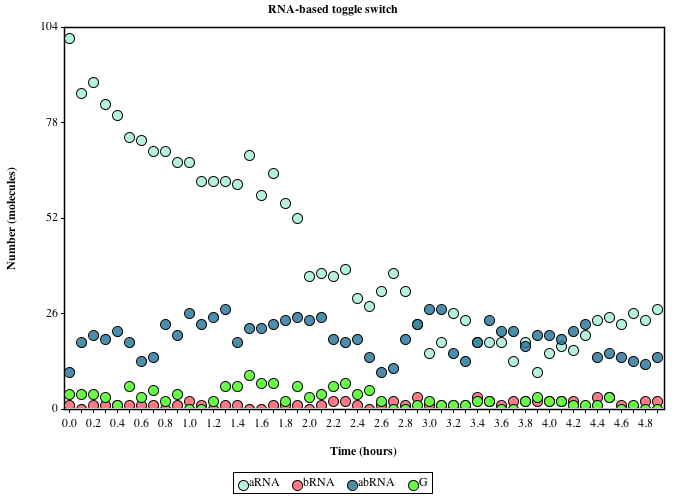
\includegraphics[scale=0.3]{RNA_based_toggle_timecourse.png}
    \end{column}
    \begin{column}{0.5\textwidth}
      \centering
      \scalebox{0.5}{
      \schemestart
      $a_{DNA}$%\phantom{I}
      \arrow{->[$k_{a_{tc}}$]}
      $a_{RNA}$\phantom{}
      \arrow{<=>[*0$k_{a_{on}}$][*0$k_{a_{off}}$]}[-90]
      $a_{RNA}\cdot b_{RNA}$
      \arrow{<=>[*0$k_{b_{on}}$][*0$k_{b_{off}}$]}[-90]
      $b_{RNA}$
      \arrow{<-[$k_{b_{tc}}$]}[180]
      $b_{DNA}$
      \arrow(@c2--){->[$k_{a_{deg}}$]}
      $\emptyset$
      \arrow(@c3--){->[$k_{ab_{deg}}$]}
      $\emptyset$
      \arrow(@c4--){->[$k_{b_{deg}}$]}
      $\emptyset$
      \schemestop    
      }
    \end{column}
  \end{columns}
\end{frame}

%------------------------------------------------
\subsection{Classic Repressilator}
\begin{frame}
\frametitle{Classic Repressilator}
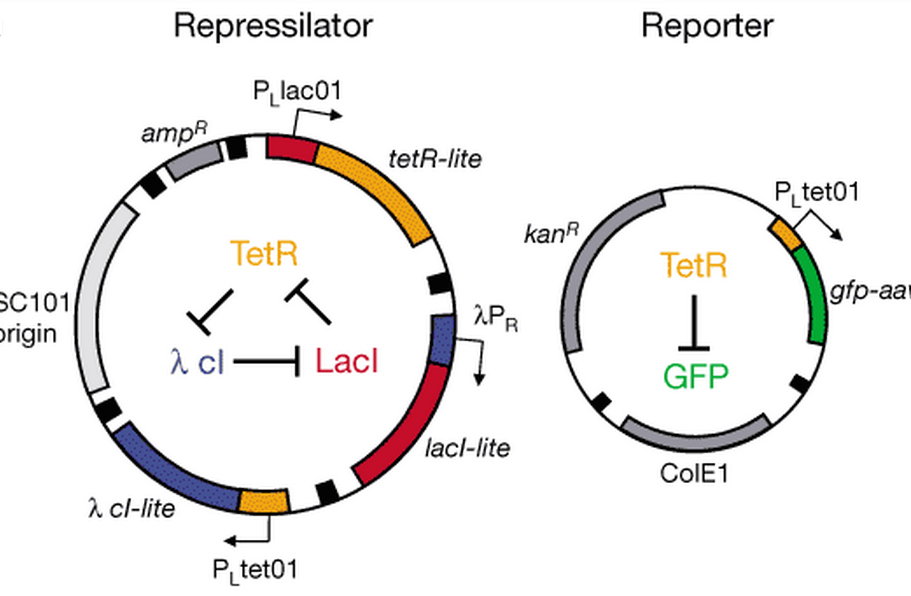
\includegraphics[width=0.5\textwidth]{repressilator_plasmids.png}
\hfill
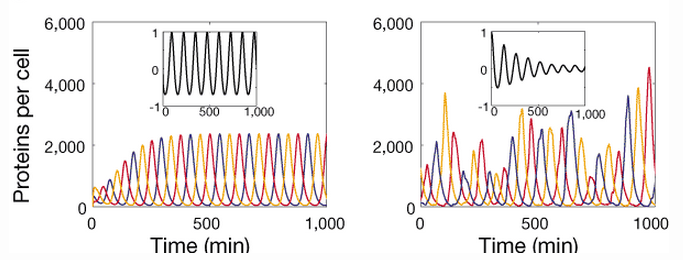
\includegraphics[width=0.5\textwidth]{repressilator_time.png}
\end{frame}
%------------------------------------------------

\subsection{Riboregulatory Repressilator}
\begin{frame}
\frametitle{Riboregulatory Repressilator}

\begin{columns}[T]
  \begin{column}{0.5\textwidth}      
    \centering
       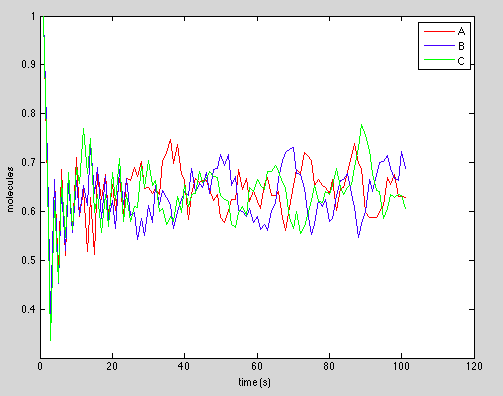
\includegraphics[scale=0.4]{repress_graph.png}
    \end{column}    
    \begin{column}{0.4\textwidth}
      \centering
      \scalebox{0.4}{
      \schemestart
      $a_{DNA}$%\phantom{I}
      \arrow{->[$k_{a_{tc}}$]}
      $a_{RNA}$\phantom{}
      \arrow{->[$k_{deg_a}$]}
      $\emptyset$
      \schemestop    
      }

      \scalebox{0.4}{
        \schemestart
        $b_{DNA}$%\phantom{I}
        \arrow{->[$k_{b_{tc}}$]}
        $b_{RNA}$\phantom{}
        \arrow{->[$k_{deg_b}$]}
        $\emptyset$
        \schemestop
      }

      \scalebox{0.4}{
        \schemestart
        $c_{DNA}$%\phantom{I}
        \arrow{->[$k_{c_{tc}}$]}
        $c_{RNA}$\phantom{}
        \arrow{->[$k_{deg_c}$]}
        $\emptyset$
        \schemestop
      }

      \scalebox{0.4}{
        \schemestart
        $a_{RNA}+b_{RNA}$%\phantom{I}
        \arrow{<=>[$k_{on_{ab}}$][$k_{off_{ab}}$]}
        $a_{RNA}\cdot b_{RNA}$\phantom{}
        \arrow{->[$k_{cleave_{a}}$]}
        $a_{RNA}$
        \schemestop
      }

      \scalebox{0.4}{
        \schemestart
        $b_{RNA}+c_{RNA}$%\phantom{I}
        \arrow{<=>[$k_{on_{bc}}$][$k_{off_{bc}}$]}
        $b_{RNA}\cdot c_{RNA}$\phantom{}
        \arrow{->[$k_{cleave_{b}}$]}
        $b_{RNA}$
        \schemestop
      }

      \scalebox{0.4}{
        \schemestart
        $c_{RNA}+a_{RNA}$%\phantom{I}
        \arrow{<=>[$k_{on_{ca}}$][$k_{off_{ca}}$]}
        $c_{RNA}\cdot a_{RNA}$\phantom{}
        \arrow{->[$k_{cleave_{c}}$]}
        $c_{RNA}$
        \schemestop
      }

    \end{column}    
  \end{columns}

\end{frame}
%------------------------------------------------

\subsection{Repressilator Comparison}
\begin{frame}
\frametitle{Repressilator Comparison}

Rate of oscillation 

Tunable:
\begin{itemize}
 \item promoter strength

 \item  strength of binding

 \item  cleavage rate - fairly fixed 
 
 \item degradation rate

\end{itemize}


\end{frame}

%------------------------------------------------

\section{Implications and further work}
\begin{frame}
\frametitle{Implications and further work}

Biocircuit-Design Automation,

Biocompiler

\begin{figure}
  \centering
  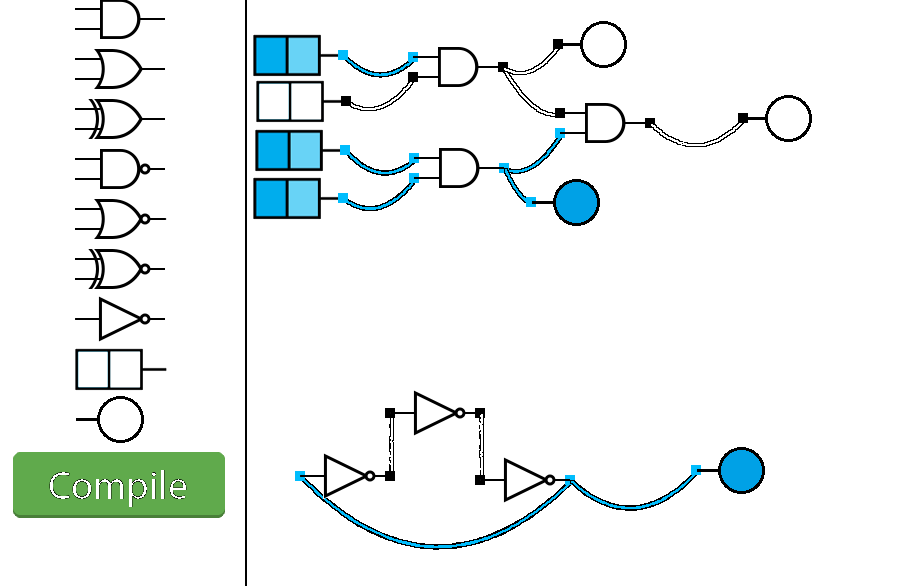
\includegraphics[scale=0.2]{repress_4and.png}
\end{figure}

\end{frame}

%------------------------------------------------

\begin{frame}
\frametitle{Thanks!}

Thanks to Sergey and Jeremy for their feedback and help throughout the course

Thanks to Adam and Ron for all your time and for giving us a solid synbio foundation

And thanks to Leslie for working out the logistics
\end{frame}
%------------------------------------------------

\begin{frame}
\frametitle{Sources}

\begin{itemize}
\item Pray, L. A.; \url{http://www.nature.com/scitable/topicpage/eukaryotic-genome-complexity-437}
\item Arkin, A. and Weiss, Ron; Principles of Synthetic Biology Fall 2013; Lecture 3
\item Carlson, Rob; DNA cost curves; \url{http://www.synthesis.cc/2011/06/new-cost-curves.html}
\item Stanton, B.C. et al.; \emph{Genomic Mining of prokaryotic repressors for orthogonal logic gates};
  \url{http://www.nature.com/nchembio/journal/vaop/ncurrent/full/nchembio.1411.html}
\item Martin, J.N., et al.; Lethal toxicity caused by expression of shRNA in the mouse striatum: implications for therapeutic design;
  \url{http://www.nature.com/gt/journal/v18/n7/full/gt201110a.html}
\item Bongarets; \emph{GFP as a Marker for Conditional Gene Expression in Bacterial Cells}
  \url{http://www.ifr.ac.uk/Safety/molmicro/pubs/bongaerts2002.pdf}
\item Anderson, J.C.; \emph{org.devicecourse Gillespie module}
\item Gillespie, Daniel T. (1977). \emph{Exact Stochastic Simulation of Coupled Chemical Reactions}. The Journal of Physical Chemistry 81 (25): 2340–2361. doi:10.1021/j100540a008.
\item Samarsky et al.; \emph{A small nucleolar RNA:ribozyme hybrid cleaves a nucleolar RNA
target in vivo with near-perfect efficiency}; \url{http://www.pnas.org/content/96/12/6609.full.pdf}
\end{itemize}

\end{frame}

%------------------------------------------------
\begin{frame}
\frametitle{Multiple Columns}
\begin{columns}[c] % The "c" option specifies centered vertical alignment while the "t" option is used for top vertical alignment

\column{.45\textwidth} % Left column and width
\textbf{Heading}
\begin{enumerate}
\item Statement
\item Explanation
\item Example
\end{enumerate}

\column{.5\textwidth} % Right column and width
Lorem ipsum dolor sit amet, consectetur adipiscing elit. Integer lectus nisl, ultricies in feugiat rutrum, porttitor sit amet augue. Aliquam ut tortor mauris. Sed volutpat ante purus, quis accumsan dolor.

\end{columns}
\end{frame}


\end{document} 